\documentclass{beamer}
\usepackage{hyperref}
\usepackage[T1]{fontenc}
\usepackage{ctex}
\UseRawInputEncoding
\usepackage{xwatermark}
% Cannot enable in Xelatex
\usepackage{pgfpages}
% \setbeameroption{hide notes} % Only slides
% \setbeameroption{show only notes} % Only notes
% \setbeameroption{show notes on second screen}

% other packages
\usepackage{latexsym,amsmath,xcolor,multicol,booktabs,calligra}
\usepackage{graphicx,listings,stackengine}

%% Enable only in Xelatex
% \usepackage{pstricks}

\author{García-Álvarez Gregorio E. , Luna-Macías Antonio J. , Tevera-Ruiz Alejandro}
\title{Reporte de Medio Término}
\subtitle{Presentación}
\institute [CINVESTAV] {Maestría en Ciencias de Robótica y Manufactura Avanzada}
\date{Robótica 1}
\usepackage{YTU}

% defs
\def\cmd#1{\texttt{\color{red}\footnotesize $\backslash$#1}}
\def\env#1{\texttt{\color{blue}\footnotesize #1}}
\definecolor{deepblue}{rgb}{0,0,0.5}
\definecolor{deepred}{rgb}{0.6,0,0}
\definecolor{deepgreen}{rgb}{0,0.5,0}
\definecolor{halfgray}{gray}{0.55}

\lstset{
    basicstyle=\ttfamily\small,
    keywordstyle=\bfseries\color{deepblue},
    emphstyle=\ttfamily\color{deepred},    % Custom highlighting style
    stringstyle=\color{deepgreen},
    numbers=left,
    numberstyle=\small\color{halfgray},
    rulesepcolor=\color{red!20!green!20!blue!20},
    frame=shadowbox,
}


\begin{document}

\begin{frame}
    \titlepage
    \begin{figure}[htpb]
        \begin{center}
            
\includegraphics[width=0.15\linewidth]{Cinvestav.jpg}
        \end{center}
    \end{figure}
    
    \begin{note}
        {Robótica 1}
    \end{note}

\end{frame}

\begin{frame}
    \tableofcontents[sectionstyle=show,subsectionstyle=show/shaded/hide,subsubsectionstyle=show/shaded/hide]
\end{frame}


\section{Introducción}

\begin{frame}{Original Template}
    \begin{itemize}[<+-| alert@+>] % 当然,除了alert,手动在里面插 \pause 也行
        \item Modify from this theme \cite{origin}
        \item Overleaf  \url{https://www.overleaf.com/latex/templates/thu-beamer-theme/vwnqmzndvwyb}
        \item GitHub Page \url{https://github.com/Trinkle23897/THU-Beamer-Theme}
    \end{itemize}
    
    \note {Write your notes.\\}
    \begin{note}
        {Write your notes here}
    \end{note}
\end{frame}



\section{Antecedentes}

\subsection{Beamer Subsection}

\begin{frame}{Beamer Features}
    \begin{itemize}
        \item More features come from  \url{https://www.latexstudio.net/archives/4051.html}
    \end{itemize}
\end{frame}

\section{Implementación}

\subsection{}



\subsection{How to use Beamer}

\begin{frame}{Formatting Samples}
    \begin{exampleblock}{Equation without numbers} 
        \begin{equation*}
            J(\theta) = \mathbb{E}_{\pi_\theta}[G_t] = \sum_{s\in\mathcal{S}} d^\pi (s)V^\pi(s)=\sum_{s\in\mathcal{S}} d^\pi(s)\sum_{a\in\mathcal{A}}\pi_\theta(a|s)Q^\pi(s,a)
        \end{equation*}
    \end{exampleblock}
    \begin{exampleblock}{Multiple equations\footnote{If containing text in equations,use $\backslash$mathrm\{\} or $\backslash$text\{\}}}
       
        \begin{align}
            Q_\mathrm{target}&=r+\gamma Q^\pi(s^\prime, \pi_\theta(s^\prime)+\epsilon)\\
            \epsilon&\sim\mathrm{clip}(\mathcal{N}(0, \sigma), -c, c)\nonumber
        \end{align}
    \end{exampleblock}
\end{frame}

\begin{frame}
    \begin{exampleblock}{Equation with numbers}
        % Taken from Mathmode.tex
        \begin{multline}
            A=\lim_{n\rightarrow\infty}\Delta x\left(a^{2}+\left(a^{2}+2a\Delta x+\left(\Delta x\right)^{2}\right)\right.\label{eq:reset}\\
            +\left(a^{2}+2\cdot2a\Delta x+2^{2}\left(\Delta x\right)^{2}\right)\\
            +\left(a^{2}+2\cdot3a\Delta x+3^{2}\left(\Delta x\right)^{2}\right)\\
            +\ldots\\
            \left.+\left(a^{2}+2\cdot(n-1)a\Delta x+(n-1)^{2}\left(\Delta x\right)^{2}\right)\right)\\
            =\frac{1}{3}\left(b^{3}-a^{3}\right)
        \end{multline}
    \end{exampleblock}
\end{frame}

\begin{frame}{Figure and Column}
    % From thuthesis user guide.
    \begin{minipage}[c]{0.3\linewidth}
    %%% DO NOT USE PSTricks in pdflatex
%         \psset{unit=0.8cm}
%         \begin{pspicture}(-1.75,-3)(3.25,4)
%             \psline[linewidth=0.25pt](0,0)(0,4)
%             \rput[tl]{0}(0.2,2){$\vec e_z$}
%             \rput[tr]{0}(-0.9,1.4){$\vec e$}
%             \rput[tl]{0}(2.8,-1.1){$\vec C_{ptm{ext}}$}
%             \rput[br]{0}(-0.3,2.1){$\theta$}
%             \rput{25}(0,0){%
%             \psframe[fillstyle=solid,fillcolor=lightgray,linewidth=.8pt](-0.1,-3.2)(0.1,0)}
%             \rput{25}(0,0){%
%             \psellipse[fillstyle=solid,fillcolor=yellow,linewidth=3pt](0,0)(1.5,0.5)}
%             \rput{25}(0,0){%
%             \psframe[fillstyle=solid,fillcolor=lightgray,linewidth=.8pt](-0.1,0)(0.1,3.2)}
%             \rput{25}(0,0){\psline[linecolor=red,linewidth=1.5pt]{->}(0,0)(0.,2)}
% %           \psRotation{0}(0,3.5){$\dot\phi$}
% %           \psRotation{25}(-1.2,2.6){$\dot\psi$}
%             \psline[linecolor=red,linewidth=1.25pt]{->}(0,0)(0,2)
%             \psline[linecolor=red,linewidth=1.25pt]{->}(0,0)(3,-1)
%             \psline[linecolor=red,linewidth=1.25pt]{->}(0,0)(2.85,-0.95)
%             \psarc{->}{2.1}{90}{112.5}
%             \rput[bl](.1,.01){C}
%         \end{pspicture}
    \end{minipage}\hspace{1cm}
    \begin{minipage}{0.5\linewidth}
        \medskip
        %\hspace{2cm}
        \begin{figure}[h]
            \centering
            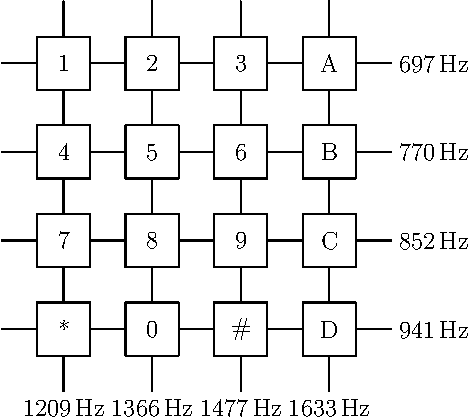
\includegraphics[height=.4\textheight]{pic/dtmf.pdf}
        \end{figure}
    \end{minipage}
\end{frame}

\begin{frame}[fragile]{\LaTeX{} Commands}
    \begin{exampleblock}{Commands}
        \centering
        \footnotesize
        \begin{tabular}{llll}
            \cmd{chapter} & \cmd{section} & \cmd{subsection} & \cmd{paragraph} \\
            Chapter & Section & Subsection & Paragraph \\\hline
            \cmd{centering} & \cmd{emph} & \cmd{verb} & \cmd{url} \\
            Centre Align & Emphasis & Verbatim & Hyperlink \\\hline
            \cmd{footnote} & \cmd{item} & \cmd{caption} & \cmd{includegraphics} \\
            Foodnote & Item & Caption & FigP\&Pic \\\hline
            \cmd{label} & \cmd{cite} & \cmd{ref} \\
            Label & Citing & Referring\\\hline
        \end{tabular}
    \end{exampleblock}
    \begin{exampleblock}{Environment Command}
        \centering
        \footnotesize
        \begin{tabular}{lll}
            \env{table} & \env{figure} & \env{equation}\\
            Table & Figure & Equation \\\hline
            \env{itemize} & \env{enumerate} & \env{description}\\
            Bullets & Numbering & Description \\\hline
        \end{tabular}
    \end{exampleblock}
\end{frame}

\begin{frame}[fragile]{\LaTeX{} Environment Command Samples}
    \begin{minipage}{0.5\linewidth}
\begin{lstlisting}[language=TeX]
\begin{itemize}
  \item A \item B
  \item C
  \begin{itemize}
    \item C-1
  \end{itemize}
\end{itemize}
\end{lstlisting}
    \end{minipage}\hspace{1cm}
    \begin{minipage}{0.3\linewidth}
        \begin{itemize}
            \item A
            \item B
            \item C
            \begin{itemize}
                \item C-1
            \end{itemize}
        \end{itemize}
    \end{minipage}
    \medskip
    \pause
    \begin{minipage}{0.5\linewidth}
\begin{lstlisting}[language=TeX]
\begin{enumerate}
  \item Class 1 
  \item Class 2
  \item Class 2
  \begin{itemize}
    \item[n+e] Student 1
  \end{itemize}
\end{enumerate}
\end{lstlisting}
    \end{minipage}\hspace{1cm}
    \begin{minipage}{0.3\linewidth}
        \begin{enumerate}
            \item Class 1
            \item Class 2
            \item Class 3
            \begin{itemize}
                \item[n+e] Student 1
            \end{itemize}
        \end{enumerate}
    \end{minipage}
\end{frame}

\begin{frame}[fragile]{\LaTeX{} Equations}
    \begin{columns}
        \begin{column}{.55\textwidth}
\begin{lstlisting}[language=TeX]
$V = \frac{4}{3}\pi r^3$

\[
  V = \frac{4}{3}\pi r^3
\]

\begin{equation}
  \label{eq:vsphere}
  V = \frac{4}{3}\pi r^3
\end{equation}
\end{lstlisting}
        \end{column}
        \begin{column}{.4\textwidth}
            $V = \frac{4}{3}\pi r^3$
            \[
                V = \frac{4}{3}\pi r^3
            \]
            \begin{equation}
                \label{eq:vsphere}
                V = \frac{4}{3}\pi r^3
            \end{equation}
        \end{column}
    \end{columns}
    \begin{itemize}
        \item Check more \href{https://en.wikipedia.org/wiki/Help:Displaying_a_formula}{\color{purple}{Here}}
    \end{itemize}
\end{frame}

\begin{frame}[fragile]
    \begin{columns}
        \column{.6\textwidth}
\begin{lstlisting}[language=TeX]
\begin{table}[htbp]
  \caption{Definition}
  \label{tab:number}
  \centering
  \begin{tabular}{cl}
    \toprule
    Word & Definition \\
    \midrule
    1 & 4.0 \\
    2 & 3.7 \\
    \bottomrule
  \end{tabular}
\end{table}
Check definition of 
Equation~(\ref{eq:vsphere}) 
in Table~\ref{tab:number}。
\end{lstlisting}
        \column{.4\textwidth}
        \begin{table}[htpb]
            \centering
            \caption{Definition}
            \label{tab:number}
            \begin{tabular}{cl}\toprule
                Eq. & Def. \\\midrule
                1 & 4.0\\
                2 & 3.7\\\bottomrule
            \end{tabular}
        \end{table}
        \normalsize Please check the definition of Equation~(\ref{eq:vsphere}) in Table~\ref{tab:number}
    \end{columns}
\end{frame}

\begin{frame}{Plotting}
    \begin{itemize}
        \item Vector: eps, ps, pdf
        \begin{itemize}
            \item METAPOST, pstricks, pgf $\ldots$
            \item Xfig, Dia, Visio, Inkscape $\ldots$
            \item Export Matlab / Excel as pdf
        \end{itemize}
        \item Bitmap: png, jpg, tiff $\ldots$
        \begin{itemize}
            \item Avoiding using bitmaps 
        \end{itemize}
    \end{itemize}

\end{frame}
\begin{frame}
  
\end{frame}

\section{Discusión}
\begin{frame}
    \begin{itemize}
        \item Year 1
        \item Year 2
        \item Year 3
        \item ...
    \end{itemize}
\end{frame}

\section{Conclusiones}

\begin{frame}

\end{frame}

\section{Referencias}

\begin{frame}[allowframebreaks]
    \bibliography{ref}
    \bibliographystyle{alpha}
    % If too many references, use this command to resize:
    % \tiny\bibliographystyle{alpha}
\end{frame}

\begin{frame}

\begin{figure}[htpb]
        \begin{center}
            
\includegraphics[width=0.15\linewidth]{Cinvestav.jpg}
        \end{center}
    \end{figure}
   
    \begin{center}
        {\Huge\calligra ¡Gracias por su atención! }
    \end{center}
   
\end{frame}

\end{document}